\chapter{Project}\glsresetall
\section{The Spatial Stokes Layer (SSL) Mean Velocity Profile}\label{sec:sslmean}
The \gls{ssl} mean streamwise velocity profile $\overline{U}\ssl\ps$ was given by \vqt, along with that of \gls{tsl}, the reference channel flow, and $\overline{U}^{+}=y^{+}$ for comparison (Figure~\ref{fig:sslmeanprofile}). We can see that at $y^{+}<10$, they all coincide to the linear profile $\overline{U}^{+}=y^{+}$, and at some point between $10<y^{+}<40$, they stop being curved on the logarithmic plot and become straight with similar slopes, indicating a logarithmic profile at higher $y^{+}$. In fact, like other \gls{dr} techniques (e.g. riblets), the \gls{dr} is noticeable as a thickening of the viscous sublayer causing an upward shift in this logarithmic portion of the mean velocity profile \cite{viotti2009,choi1989,luchini1996}. 

\begin{figure}[htbp]
	\centering
	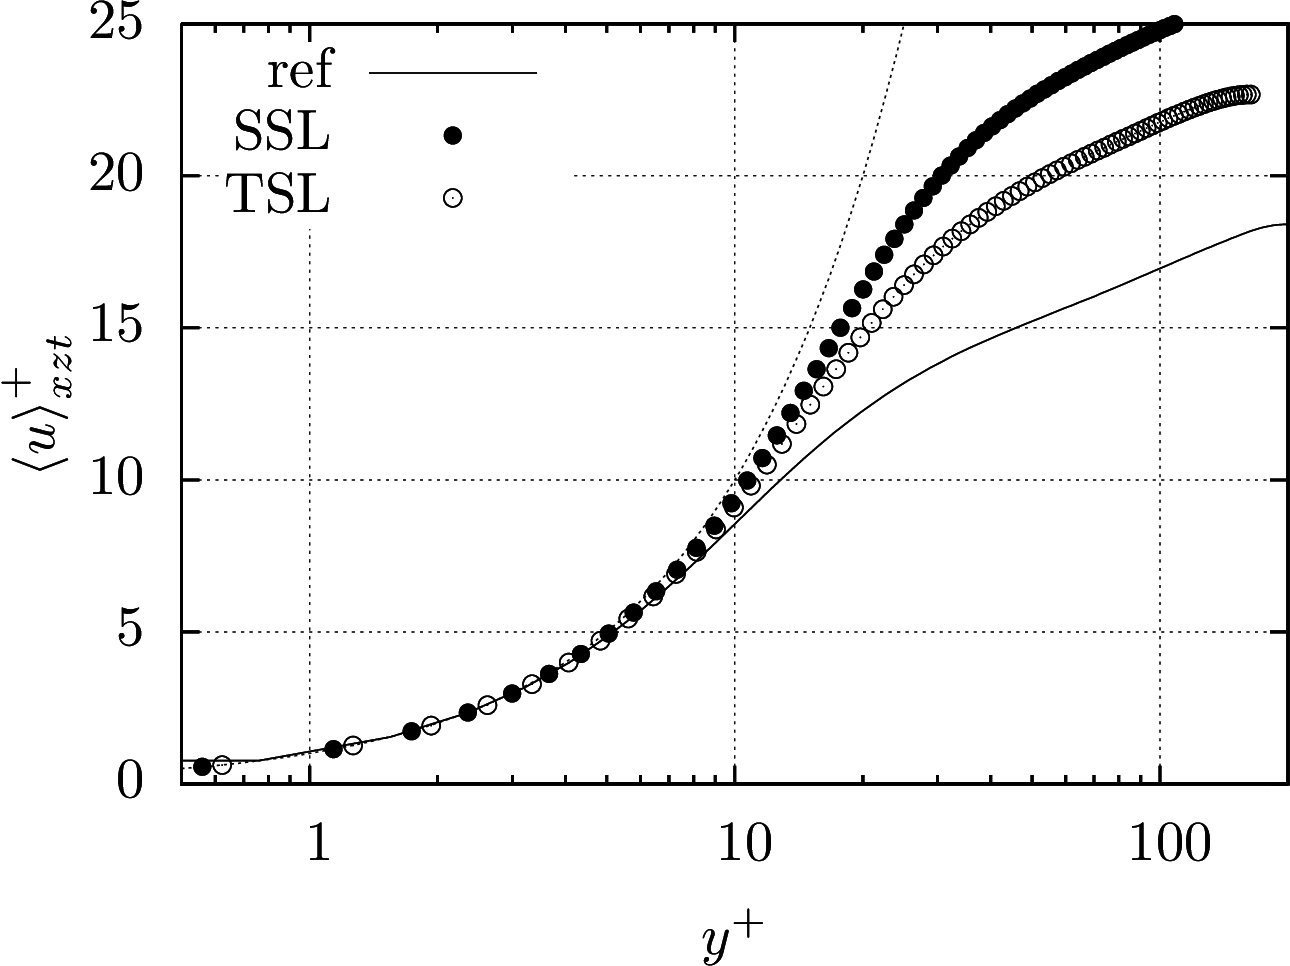
\includegraphics[width=0.5\linewidth]{project/fig/sslmeanprofile.png}
	\caption[Streamwise mean velocity profiles of SSL and reference flow]{Streamwise mean velocity profiles in wall units averaged in $x$-$z$ space, time, and phase ($\overline{U}^{+}\equiv \left<u \right>^{+}_{xzt}$) for \gls{ssl}, \gls{tsl}, the reference flow, and $\overline{U}^{+}=y^{+}$ (dotted line) for comparison \cite{viotti2009}.}
	\label{fig:sslmeanprofile}
\end{figure}

In order to see the differences more clearly, the  \gls{ssl} and refence flow data from Figure~\ref{fig:sslmeanprofile} were digitised using the web app webplotdigitiser. 

\begin{figure}[htbp]
	\centering
	\subfigure[Curve fit.]{
		\label{fig:sslmpcf}
        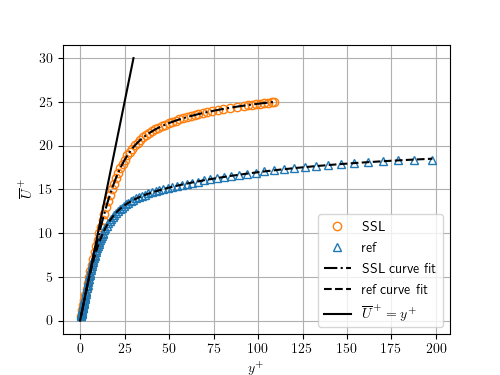
\includegraphics[width=0.485\linewidth]{project/fig/sslmeanprofilelin.png}}
	\subfigure[Estimated Logarithmic profiles.]{
		\label{fig:sslmpest}
		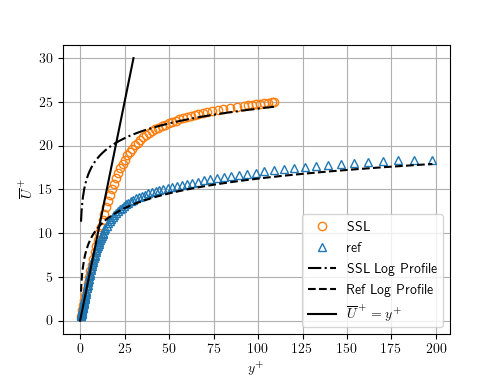
\includegraphics[width=0.485\linewidth]{project/fig/sslmeanprofileest.png}}
		\caption{Both plots show data on the mean streamwise velocity profiles of \gls{ssl} (orange-circle) and the reference flow (blue-triangles) were digitised from \textcite{viotti2009} and plotted on a linear scale, as well as $\overline{U}^+=y^+$ (solid-line). }
	\label{fig:sslmplin}
\end{figure}

